\documentclass{article}

\usepackage{amsmath}
\usepackage{amsfonts}
\usepackage{amssymb}

\usepackage{mathenv}

\def\nbOne{{\mathchoice {\rm 1\mskip-4mu l} {\rm 1\mskip-4mu l}
{\rm 1\mskip-4.5mu l} {\rm 1\mskip-5mu l}}}

\usepackage{vmargin}
\setmarginsrb{2.5cm}{2.5cm}{2.5cm}{2.5cm}{0cm}{0cm}{0cm}{0cm}

\usepackage[utf8]{inputenc}

\usepackage[french]{babel}
\selectlanguage{french}

\usepackage{enumerate}
\usepackage{color}
\usepackage{graphicx}
\graphicspath{{img/}} 

% Commandes personnelles %

\newcommand{\R}{\mathbb{R}}
\newcommand{\Z}{\mathbb{Z}}
\newcommand{\N}{\mathbb{N}}
\newcommand{\ab}{\textbf{arbre binaire }}
\newcommand{\abr}{\textbf{arbre binaire de recherche }}
\newcommand{\abrb}{\textbf{arbre binaire de recherche}}
\newcommand{\algo}[1]{\textcolor{darkblue}{\textbf{#1}}}
\newcommand{\param}[1]{\textcolor{darkred}{#1}}

\definecolor{darkred}{rgb}{0.85,0,0}
\definecolor{darkblue}{rgb}{0,0,0.7}
\definecolor{darkgreen}{rgb}{0,0.7,0}

\DeclareMathAlphabet{\mathpzc}{OT1}{pzc}{m}{it}

\title{\textbf{\textcolor{darkblue}{Structures de données II.}}}
\author{\textit{Xavier Dubuc}}

\begin{document}

\maketitle

\hbox{\raisebox{0.4em}{\vrule depth 0.4pt height 0.4pt width 10cm}}

\tableofcontents % Affiche la table des matiéèes

\hbox{\raisebox{0.4em}{\vrule depth 0.4pt height 0.4pt width 10cm}}

\section{Chapitre 2 - Les arbres}

\subsection{Propriétés des arbres.}

\begin{enumerate}
\item Si $T$ est un \ab à $n$ noeuds et de hauteur $h$, alors on a : \\
- $h \leq n \leq 2^k-1 \\$
- $\log_2(n+1) \leq h \leq n \ \ \ $(Corollaire $h$ est en $O(n)$)

\item Si $T$ est un \ab à $n$ noeuds et de hauteur $h$, soit $n_I$ son nombre de noeuds internes et $n_F$
son nombre de feuilles, alors on a : \\
- $h-1 \leq n_I \leq 2^{k-1}-1 \\$
- $1 \leq n_F \leq 2^{k-1}$

\item $C(t)$ complété de $T$, \ab de recherche, si $T$ a $n$ noeuds, alors $C(T)$ a $2n+1$ noeuds (corollaire, $T$ a $n+1$
références vides).

\underline{Définition récursive} : Profondeur d'un noeud :
\begin{itemize}
\item Profondeur de la racine : 0
\item Si un noeud a une profondeur $p$, alors ses fils ont une profondeur de $p+1$.
\end{itemize}

\underline{Définition} : $T$, \ab, $C(T)$ son complété, on définit :

\begin{itemize}
\item \textit{Internal path length} : $I(T)$ : somme des profondeurs des noeuds internes de T.
\item \textit{External path length} : $E(T)$ : somme des profondeurs des feuilles de T.
\end{itemize}
 
\underline{Exemple} : 

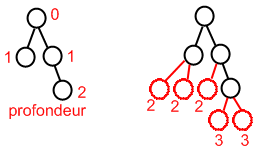
\includegraphics[width=200px]{img1.png}

$I(T) = 0+1+1+2 = 4 \\
E(T) = 2+2+2+3+3 = 12$

\item $E(T) = I(T) + 2n$ et $(n+1) \log_2\left\{\dfrac{(n+1)}{4}\right\} < I(T) \leq \dfrac{n(n-1)}{2}$ \\

\underline{Preuve} : \\
Prouvons que $E(T) = I(T) + 2n$, calculons de 2 façons $\sideset{}{_{v\ noeuds\ de\ C(T)}}\sum{prof(v)}$ : \\
(1) $ = \sideset{}{_{v\ noeuds\ internes\ de\ C(T)}}\sum{prof(v)} + \sideset{}{_{v\ feuilles\ de\ C(T)}}\sum{prof(v)} $ \\
    $\ = \sideset{}{_{v\ noeuds\ de\ T}}\sum{prof(v)} + \sideset{}{_{v\ feuilles\ de\ C(T)}}\sum{prof(v)} = I(T)+E(T)$ \\

(2) $ = prof(racine) + \sideset{}{_{v\ noeuds\ de\ T}}\sum{2\left(prof(v)+1\right)} = 0 + 2
\sideset{}{_{v\ noeuds\ de\ T}}\sum{prof(v)} + 2n$

\underline{\textit{Explications}} : tout noeud de $C(T)$ est le fils d'un noeud interne de $C(T)$ c'est-à-dire un noeud 
de $T$ (sauf la racine), de plus, tout noeud interne de $C(T)$ a 2 fils par définition.

(1)$=$(2) $\Rightarrow I(T)+E(T) = 2n+2I(T) \Rightarrow \textcolor{darkred}{E(T) = I(T) + 2n}$ \\

Prouvons que $(n+1) \log_2\left\{\dfrac{(n+1)}{4}\right\} < I(T) \leq \dfrac{n(n-1)}{2}$, \\

Comme pour la hauteur, on va s'interesser à un arbre qui a un nombre minimum de noeuds, et à un arbre qui a un nombre
maximum de noeuds.

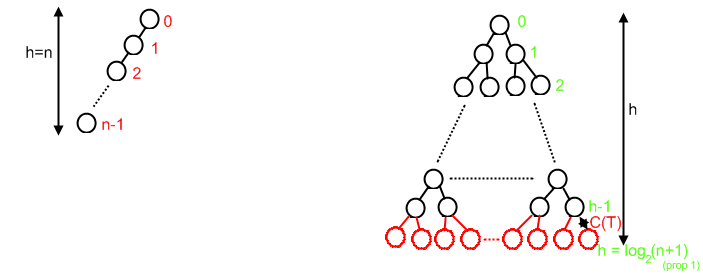
\includegraphics[width=300px]{img2.png}

\underline{Premier dessin} : \\ $I(T) = 0+1+...+(n-1) = \dfrac{(n-1)n}{2}$ \\
\underline{Second dessin} : \\ $I(T) = E(T) - 2n$ \\
$ = \sideset{}{_{v\ noeuds\ de\ C(T)}}\sum{prof(v)} = \sideset{}{_{v\ feuilless\ de\ C(T)}}\sum{\log_2(n+1)}$ \\
$ = (n+1)\log_2(n+1)-2n$ \\

\underline{En général : } \\
$(n+1)\log_2(n+1)-2n \leq I(T) \leq \dfrac{(n-1)n}{2} \\
(n+1)\log_2(n+1)-2(n+1) < I(T)  \\ 
(n+1) \left[ \log_2(n+1) - 2 \right] < I(T) \\
(n+1) \left[ \log_2(n+1) - \log_2(4) \right] < I(T)  \\
(n+1) \log_2\left(\dfrac{(n+1)}{4} \right) < I(T) \\$

\underline{Commentaires : } \\

$h$ a une complexité comprise entre $\log_2n$ et $n$ et I(T) entre $n\ \log_2n$ et $n^2$.

\end{enumerate}

\section{Chapitre 3 - Arbres binaires de recherche}

\underline{Définition} : il s'agit d'un arbre binaire(y compris l'arbre vide) tel que pour tout noeud, la donnée qui 
\indent s'y trouve est $<$ à toutes les données du sous-arbre droit et $>$ à celles du sous-arbre gauche.

\underline{Exemple} : 

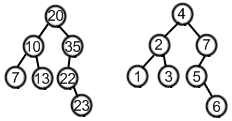
\includegraphics{img3.png}

\subsection{Hauteur} Au pire, la hauteur $h$ est en $O(n)$ (voir la première propriété)

\subsection{Recherche d'une donnée $k$ dans un \ab de recherche.}

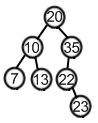
\includegraphics[width=100px]{img4.png}

\underline{\textcolor{darkgreen}{Recherche avec succès : $k=22$}} \\
\textit{A chaque noeud rencontré, on laisse tomber l'un des 2 sous arbres. (recherche dichotomique) Ici, contrairement
au calcul de la hauteur, on ne visite qu'une partie des noeuds. (placé sur un chemin partant de la racine).}\\
\indent\underline{\textcolor{darkred}{Recherche avec succès : $k=12$}} \\
\textit{Le chemin suivi aboutit à une référence vide $\rightarrow$ $12$ n'est pas présent.} \\
 
Nous allons développer un algorithme basé sur la définition récursive des arbres binaires de recherche, \\
\underline{Cas de base} : $T$, arbre vide, $k$ n'est donc pas présent. \\
\underline{Cas général} : $T$ est un arbre contenant une donnée $x$ et 2 sous-arbres $T_1$ et $T_2$.\\
\begin{itemize}
 \item $k=x$, $k$ est présent, on l'a trouvé.
 \item $k>x$, $k$ est présent dans $T$ si et seulement si $k$ est présent dans $T_2$ (l'arbre de droite).
 \item $k<x$, $k$ est présent dans $T$ si et seulement si $k$ est présent dans $T_1$ (l'arbre de gauche).
\end{itemize}

\subsubsection{Algorithme}

Algorithme \textbf{Recherche}(\textcolor{darkred}{T},\textcolor{darkred}{k}) \\
\underline{Entrée} : \textit{\textcolor{darkred}{T}, \ab de recherche.} \\
\indent\indent  \textit{\textcolor{darkred}{k}, une donnée.} \\
\underline{Sortie} : \textit{booléen vrai ssi \textcolor{darkred}{k} est dans \textcolor{darkred}{T}}.\\
$Si\ EstVide(\textcolor{darkred}{T})\ alors\ retourner\ \mathbf{faux} \\
 Sinon\ Si\ (\textcolor{darkred}{T}_{data} = \textcolor{darkred}{k})\ alors\ retourner\ \mathbf{vrai} \\
 \indent Sinon\ Si\ (\textcolor{darkred}{k} > \textcolor{darkred}{T}_{data})\ alors\ retourner\ 
\textcolor{darkblue}{\mathbf{Recherche}}(\textcolor{darkred}{T}_{right},\textcolor{darkred}{k}) \\
 \indent \indent Sinon\ retourner\ \textcolor{darkblue}{\mathbf{Recherche}}
(\textcolor{darkred}{T}_{left},\textcolor{darkred}{k})$

\subsubsection{Complexité dans le pire des cas}

\begin{itemize}
\item \underline{Recherche avec succès} \\
Recherche de $k$ dans une feuille située le plus bas possible dans l'arbre : \\
\indent - nombre de noeuds visités : $h$ \\
\indent - coût local par noeud : $O(1)$ \\
\indent - pas de références visitées. \\
$\rightarrow h*O(1) = O(h) = O(n)$ la même complexité que pour les listes triées mais en pratique, le comportement est
meilleur que celui des listes.

\item \underline{Recherche avec échec} \\

Identique mis à part un travail en $O(1)$ pour traiter la seule référence vide visitée, ce qui ne modifie pas la complexité
globale, on en tire donc les mêmes conclusions.

\end{itemize}

\subsection{Insertion d'une donnée $k$ dans un \ab de recherche.}

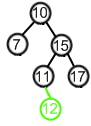
\includegraphics{img5.png}

\noindent 1) Rechercher l'endroit où insérer \\
2) Insertion proprement dit de la donnée à l'endroit repéré. \\

\textbf{\underline{Raisonnement} :} \\
$T$,$k$ entrées ; $T'$ sortie (\ab de recherche résultant de l'insertion de $k$ dans $T$) \\
\underline{Cas de base} : \textit{T arbre vide $\rightarrow T'$ sera un arbre composé d'un seul maillon contenant $k$.} \\
\underline{Cas de général} \textit{$T$ est un arbre contenant une donnée $x$ et 2 sous-arbres $T_1$ et $T_2$.} \\
\begin{itemize}
 \item $k=x$, $k$ est déjà présent, $T'=T$.
 \item $x<k$, $k$ doit être inséré à droite.
 \item $x>k$, $k$ doit être inséré à gauche.
\end{itemize}

\subsubsection{Algorithme}

Algorithme \textbf{Insertion}(\textcolor{darkred}{$T$},\textcolor{darkred}{$k$}) \\
\underline{Entrée} : \textit{\textcolor{darkred}{$T$}, \ab de recherche.} \\
\indent\indent  \textit{\textcolor{darkred}{$k$}, une donnée.} \\
\underline{Sortie} : \textit{\textbf{$T'$}}.\\
$Si\ EstVide(\textcolor{darkred}{T})\ alors\ retourner\ CreationNoeud(\textcolor{darkred}{k}) \\
Sinon\ Si\ (\textcolor{darkred}{T}_{data} = k)\ alors\ retourner\ \textcolor{darkred}{T} \\
\indent Sinon\ Si\ (\textcolor{darkred}{T}_{data} < k)\ alors\ T_{right} \leftarrow 
\textcolor{darkblue}{\textbf{Insertion}}(\textcolor{darkred}{T}_{right},\textcolor{darkred}{k}) \\
\indent\indent\indent\indent\indent\indent\indent\indent\indent Retourner\ \textcolor{darkred}{T} \\
\indent\indent Sinon\ \textcolor{darkred}{T}_{left} \leftarrow 
\textcolor{darkblue}{\textbf{Insertion}}(\textcolor{darkred}{T}_{left},\textcolor{darkred}{k}) \\
\indent\indent\indent\indent retourner\ \textcolor{darkred}{T}$ \\

\newpage

Algorithme \textbf{InsertionBis}(\textcolor{darkred}{$T$},\textcolor{darkred}{$k$}) \\
\underline{Entrée} : \textit{\textcolor{darkred}{$T$}, \ab de recherche.} \\
\indent\indent  \textit{\textcolor{darkred}{$k$}, une donnée.} \\
\underline{Sortie} : / (\textit{\textcolor{darkred}{$T$} modifié)}.\\
$Si\ EstVide(\textcolor{darkred}{T})\ alors\ 
CreerNoeudBis(\textcolor{darkred}{T},\textcolor{darkred}{k}) \\
Sinon\ Si (\textcolor{darkred}{T}_{data} < k)\ alors\ \textcolor{darkblue}{\textbf{InsertionBis}}
(\textcolor{darkred}{T}_{right},\textcolor{darkred}{k}) \\
\indent\indent Sinon\ Si\ (\textcolor{darkred}{T}_{data} > k)\ alors\ \textcolor{darkblue}{\textbf{InsertionBis}}
(\textcolor{darkred}{T}_{left},\textcolor{darkred}{k}) \\$ 

\subsubsection{Complexité dans le pire des cas}

\noindent Insertion $=$ recherche $+$ travail complémentaire, en cas de recherche avec succès, il n'y aucun travail
complémentaire, on obtient donc du $O(h)$, quant au cas de la recherche avec échec, un travail supplémentaire en
$O(1)$ est accompli, ce qui ne modifie pas la complexité globale qui reste en $O(h)$.

\subsection{Suppression d'une donnée dans un \ab de recherche.}

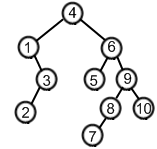
\includegraphics{img6.png}

\noindent Si on veut supprimer $\mathbf{11}$, il faut faire une recherche, se rendre compte que $\mathbf{11}$ n'est pas dans
l'arbre et ne rien faire. \\
Si on veut supprimer $\mathbf{7}$, $\mathbf{7}$ est dans une feuille, il faut supprimer la feuille. \\
Si on veut supprimer $\mathbf{1}$, $\mathbf{1}$ est dans un noeud ayant un sous arbre droit, il faut donc supprimer le noeud
contenant $\mathbf{1}$ et rattacher le sous-arbre comme sous-arbre gauche du père du noeud contenant $\mathbf{1}$.\\

\noindent \underline{Autre exemple} : \\


\includegraphics{img7.png}

\noindent Si on veut supprimer $\mathbf{2}$, $\mathbf{2}$ est dans une feuille, il faut supprimer la feuille. \\
Si on veut supprimer $\mathbf{3}$, $\mathbf{3}$ est dans un noeud ayant un sous arbre droit, il faut donc supprimer le noeud
contenant $\mathbf{3}$ et rattacher le sous-arbre comme sous-arbre gauche du père du noeud contenant $\mathbf{3}$.\\
Si on veut supprimer $\mathbf{4}$, on peut appliquer 2 idées : \\

\underline{1ère idée} : On supprime le noeud contenant $\mathbf{4}$ et on raccroche son sous-arbre gauche comme sous-arbre 
gauche de la feuille la plus à gauche du sous-arbre droit.

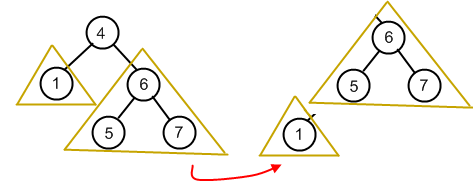
\includegraphics{img8.png}

$\rightarrow$ Ce n'est pas une bonne idée, en effet, l'arbre va tendre vers une liste, tout s'ajoutant sur la gauche.

\underline{2ème idée} : On remplace la donnée à supprimer par une autre donnée. \textit{($max(T_{left})$ ou $min(T_{right})$
en l'occurence)}

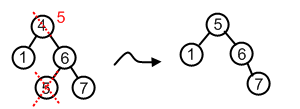
\includegraphics{img9.png}

\textit{\underline{Remarque}} : Le minimum utilisé est une feuille ou un noeud qui possède un sous-arbre droit, la 
suppression de ce noeud est donc «facile». \\

\noindent\underline{\textbf{En gros}} : la suppression se déroule en 3 étapes :
\begin{enumerate}
\item Trouver la donnée à supprimer (cf \textit{recherche})
\item Repérer le cas :
  \begin{itemize}
   \item Suppression d'une feuille.
   \item Suppression d'un noeud possédant 1 fils.
   \item Suppression d'un noeud possédant 2 fils.
  \end{itemize}
\item Si on se trouve dans le dernier cas, il faut effectuer la recherche du minimum et le remplacement de données.
\end{enumerate}

\noindent\underline{Raisonnement général} : nous allons résoudre ce problème grace à 3 algorithmes différents, l'un permettant de
supprimer la racine d'un arbre, l'un permettant de supprimer le minimum d'un arbre et faire l'échange des données ainsi
qu'un dernier supprimant les feuilles et appellant les 2 autres algorithmes dans le cas où l'argument ne serait pas une
feuille.

\subsubsection{Premier Algorithme}

\noindent\underline{Entrée} : \textit{$T$, \abr et $k$ une donnée.} \\
\underline{Sortie} : \textit{$T'$, \abr résultant de la suppression de $k$ dans $T$.} \\

\noindent \underline{Cas de base} : $T$ est un arbre vide, ce qui signifie que $k$ n'est pas dans $T$, $T'$ est donc l'arbre
vide. \\
\noindent \underline{Cas général} : $T$ est un arbre contenant une donnée $x$ et possédant un fils gauche, $T_1$, et un fils
droit, $T_2$ et on suppose que l'on peut calculer $T'_1$ et $T'_2$ les arbres résultants de la suppression de $k$ dans $T_1$
et $T_2$ respectivement. 3 cas de figure : 

\begin{itemize}
\item $k>x$ : $T'$ sera l'arbre contenant $x$, ayant $T_1$ comme fils gauche et $T'_2$ comme fils droit.
\item $k<x$ : $T'$ sera l'arbre contenant $x$, ayant $T'_1$ comme fils gauche et $T_2$ comme fils droit.
\item $k=x$ : On a trouvé $k$, on appelle le second algorithme qui va s'occuper de le supprimer. \\
\end{itemize}

\noindent Algorithme \textbf{Suppression}(\param{$T$},\param{$k$}) \\
\underline{Entrée} : \textit{\param{$T$}, \abrb.} \\
\indent\indent  \textit{\textcolor{darkred}{$k$}, une donnée.} \\
\underline{Sortie} : \textit{/ (\param{$T$} modifié en \textbf{$T'$})}.\\
\textit
{
Si (non \algo{isEmpty}(\param{$T$})) alors \\
\indent Si ($\param{k}=\param{T}_{data}$) alors \algo{SuppressionRacine}(\param{$T$}) \\
\indent Sinon Si ($\param{k}>\param{T}_{data}$) alors 
\algo{Suppression}($\param{T}_{right},\param{k}$) \\
\indent\indent\indent Sinon \algo{Suppression}($\param{T}_{left},\param{k}$) \\
} 

\subsubsection{Second Algorithme}

\noindent\underline{Entrée} : \textit{$T$, \abr non-vide.} \\
\underline{Sortie} : \textit{$T''$, \abr résultant de la suppression de la racine de $T$.} \\

\noindent\underline{Cas de base} : $T$ est une feuille, $T''$ est donc un arbre vide. \\
\underline{Cas général} : 3 cas de figure : \\
\begin{enumerate}[a)]
 \item $T$ est un arbre contenant une donnée $k$ et possédant un sous-arbre \textbf{gauche}, $T_1$, qui est un \abr;
$T''$ est donc $T_1$, en effet, si on supprime la racine, il ne reste plus que $T_1$.
 \item $T$ est un arbre contenant une donnée $k$ et possédant un sous-arbre \textbf{droit}, $T_2$, qui est un \abr;
$T''$ est donc $T_2$, en effet, si on supprime la racine, il ne reste plus que $T_2$.
 \item $T$ est un arbre contenant une donnée $k$ et possédant \textbf{2 fils}, dans ce cas on fera appel au 3ème algorithme.

On va construire $T''$, l'arbre dont la racine sera $\min{(T_2)}$, le fils gauche sera $T_1$ et le fils droit $T'''_2$
l'arbre résultant de la suppression de $\min{(T_2)}$ dans $T_2$. $T''$ est bien un \abrb. \\
En effet : \\
\underline{Avant la suppression}, on a $T_1$,$T_2$ 2 arbres binaires de recherche, on a donc la relation $T_1<k<T_2$ 
ou encore $T_1<k<min(T_2)<T'''_2$, \\
\underline{Après la suppression}, on a $T_1$ et $T'''_2$ 2 arbres binaires de recherche \textit{(par le 3ème algorithme)}
et on a bien $T_1 < min(T_2) < T'''_2$, ce qui implique que, par définition, $T''$ est un \abrb. \\
\end{enumerate}

\noindent Algorithme \textbf{SuppressionRacine}(\param{$T$}) \\
\underline{Entrée} : \textit{\param{$T$}, \abrb non-vide.} \\
\underline{Sortie} : \textit{/ (\param{$T$} modifié en \textbf{$T''$})}.\\
\textit
{
Si \algo{isLeaf}(\param{$T$}) alors \param{$T$} $\leftarrow$ arbre vide\\
\indent Sinon Si (\algo{isEmpty}($\param{T}_{right}$) alors \param{$T$} $\leftarrow \param{T}_{left}$ \\
\indent\indent Sinon Si (\algo{isEmpty}($\param{T}_{left}$) alors \param{$T$} $\leftarrow \param{T}_{right}$ \\
\indent\indent\indent\indent Sinon min $\leftarrow$ \algo{SuppressionMin}($\param{T}_{right}$) \\
\indent\indent\indent\indent\indent\indent $\param{T}_{data} \leftarrow$ min
}

\subsubsection{Troisième Algorithme}

\noindent\underline{Entrée} : \textit{$T$, \abr non-vide.} \\
\underline{Sortie} : \textit{$\min{(T)}$ ($T$ modifié en $T'''$ \abr résultant de la suppression du minimum de $T$.} \\

\noindent\underline{Cas de base} : $T$ est une feuille et contient une donnée $x$, $\min{(T)}\leftarrow x$ et 
$T'''\leftarrow$ arbre vide.\\
\underline{Cas général} : 3 cas de figure : \\
\begin{enumerate}[a)]
 \item $T$ est un arbre contenant une donnée $x$ et possédant un sous-arbre \textbf{gauche}, $T_1$, qui est un \abr;
on a donc $\min{(T)} \leftarrow \min{(T_1)}$ et $T''' \leftarrow T$ ($T$ sera modifié par l'appel récursif sur $T_1$).
 \item $T$ est un arbre contenant une donnée $x$ et possédant un sous-arbre \textbf{droit}, $T_2$, qui est un \abr;
on a donc $\min{(T)} \leftarrow x$ et $T''' \leftarrow T_2$
 \item $T$ est un arbre contenant une donnée $x$ et possédant \textbf{2 fils}, $\rightarrow$ idem que le cas a).
\end{enumerate}

\textbf{\underline{Remarque} :} \textit{On peut regrouper les cas a) et c) ainsi que le cas de base et le cas b)}. \\

\noindent Algorithme \textbf{SuppressionMin}(\param{$T$}) \\
\underline{Entrée} : \textit{\param{$T$}, \abr non-vide.} \\
\underline{Sortie} : \textit{Minimum de \param{$T$} (\param{$T$} modifié en $T'''$)}.\\
\textit
{
Si \algo{isEmpty}(\param{$T_{left}$}) alors min $\leftarrow \param{T}_{data}$ \\
\indent\indent\indent\indent\indent\indent\indent\indent \param{$T$} $\leftarrow \param{T}_{right}$ \\
Sinon min $\leftarrow$ \algo{SuppressionMin}($\param{T}_{left}$)\\
Retourner min.
}

\subsubsection{Complexité dans le pire des cas}

\begin{enumerate}
\item \underline{Pire des cas où seul le premier algorithme est exécuté}. \\
Vu que le second algorithme ne doit pas être exécuté, on a que $k\not\in T$, on effectue donc une recherche avec échec, et
dans le pire des cas la complexité d'un tel algorithme est en $O(h)$ (Vu plus tôt dans le cours). \\

\item \underline{Pire des cas où seuls les 2 premiers algorithmes sont exécuté}. \\

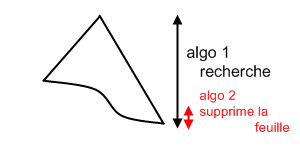
\includegraphics[height=150px]{img10.png}

Du fait que le second algorithme s'exécute, on peut conclure que $k\in T$ ; le pire des cas sera le cas où on visite le plus
de noeuds car le coût est le même pour chaque cas. On considère donc le cas où $k$ est la feuille la plus basse de $T$. Pour
ces 2 algorithmes, on visite $h$ noeuds avec une complexité en $O(1)$ et aucune références vides. Au total, on a donc une
complexité dans le pire des cas en $O(h)$. \\

\item \underline{Pire des cas où les 3 algorithmes sont exécutés}. \\

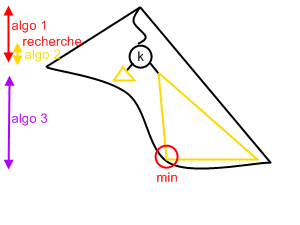
\includegraphics[height=150px]{img11.png}

Dans cette configuration, on a que $k\in T$ et que $k$ possède 2 fils non-vides. Le pire des cas sera lorsque le sous-arbre
droit de $k$ possèdera son minimum le plus en bas à gauche possible. Pour ces 3 algorithmes, on visitera $h$ noeuds avec un
coup en $O(1)$, ce qui au final reviendra à une complexité en $O(h)$. \\
\end{enumerate}

\noindent\textbf{Dans tous les cas de figure, l'algorithme a une complexité en $O(h) = O(n)$.}

\subsection{Tri de données}

Il existe une façon de trier des données à l'aide des \abrb, la voici : \\
\begin{enumerate}
\item Insérer une à une les données dans un \abr initialement vide.
\item Lire cet arbre de manière infixe.
\end{enumerate}

\subsubsection*{Complexité}

\begin{enumerate}
 \item Création \abr vide. $\rightarrow \mathbf{O(1)}$
 \item Insertions $\rightarrow n*O(h)$ ($h$ est la hauteur courante, elle est majorée par $h_{fin}$ la hauteur de l'arbre
 final), on a donc comme complexité : $\mathbf{O(n*h_{fin}) = O(n^2)}$.
 \item Lecture infixe $\rightarrow \mathbf{O(n)}$.
\end{enumerate}

\noindent\underline{Au total} : $O(1)+O(n^2)+O(n)=\mathbf{O(n^2)}$ pour trier, ce qui n'est pas mieux qu'une liste. \\

\noindent\underline{Résumé} : \\

\begin{tabular}{|*{3}{c|}}
\hline
\textbf{Algorithme} & \textbf{Listes triées} & \textbf{Arbres binaires de recherche} \\
\hline
Recherche & $O(n)$ & $O(h)$ \\
\hline
Insertion & $O(n)$ & $O(h)$ \\
\hline
Suppression & $O(n)$ & $O(h)$ \\
\hline
Tri & $O(n^2)$ & $O(n*h)$ \\
\hline
\end{tabular}

\textit{(Au pire, $h = O(n)$)} \\

En pratique, $h \neq O(n)$, on va s'interesser à la complexité en moyenne ; on était arrivé à la conclusion qu'en cas de 
recherche dans des listes triées, que ce soit avec succès ou échec, le nombre de comparaisons en moyenne était de
$\dfrac{n}{2}$. On va maintenant voir que dans le cas des \abrb, $h \sim \log_2n$, ce qui est un résultat positif car on a
vu que $\log_2(n+1) \leq h \leq n$ et donc on est plus proche de la borne inférieure que la borne supérieur (en moyenne).

\noindent Si on compte le nombre de comparaisons en moyenne, lors d'une recherche avec succès on compte $2 \ln{(n)}$ et lors
d'une recherche avec échec $2 \ln{(n)} + 2$. Ce qui est très inférieur au $\dfrac{n}{2}$ des listes triées ! \\

\underline{Hypothèses de travail pour les \abr}. \\

On va considérer $n$ données \textbf{différentes}. Lors de l'insertion dans l'arbre binaire, selon l'ordre des données, on
peut les insérer de $n!$ façons différentes ce qui implique $n!$ façon de créer un \abrb. On émet dès lors l'hypothèse que
les probabilités de travailler avec l'un des $n!$ \abr ainsi créés sont toutes les mêmes. \\

\noindent\underline{Exemple} : $n=3$\\ 

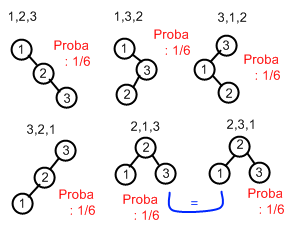
\includegraphics[height=150px]{img12.png}

\underline{Observation} : La probabilité d'avoir $k$ comme racine = $\dfrac{1}{n}$ (car être la racine de l'arbre est 
équivalent au fait d'être la première donnée parmis les n). En effet, dans le cas où $k$ est en tête de liste, le flot de
données peut être vu comme : ($k$, \textit{une des $(n-1)!$ permutations possibles entre les éléments restants}) ; de plus,
la probabilité de choisir l'un des arbres est de $\dfrac{1}{n!}$. En multipliant ces 2 probabilités, on obtient la 
probabilité pour que $k$ soit racine $\rightarrow \dfrac{(n-1)!}{n!} = \dfrac{1}{n} $.

\end{document}